% Esta es la clase que utilizamos para tomar apuntes en las asignaturas de mates y ya estoy acostumbrado a usarla. No tiene muchas cosas nuevas mas que el estilo (que podemos cambiarlo) y la cabecera y eso... Ya es el formato con el que entrego todo pero se puede usar otro si prefieres. Creo que esta basado en report (y sino en article).

\documentclass[nochap]{apuntes}

\title{Memoria Práctica 3}
\author{Víctor de Juan, Alberto Parramón, Mounaime Mellouk}
\date{C1}


% Paquetes adicionales

% --------------------
\definecolor{javared}{rgb}{0.6,0,0} % for strings
\definecolor{javagreen}{rgb}{0.25,0.5,0.35} % comments
\definecolor{javapurple}{rgb}{0.5,0,0.35} % keywords
\definecolor{javadocblue}{rgb}{0.25,0.35,0.75} % javadoc

\lstset{language=Java,
basicstyle=\ttfamily,
keywordstyle=\color{javapurple}\bfseries,
stringstyle=\color{javared},
commentstyle=\color{javagreen},
morecomment=[s][\color{javadocblue}]{/**}{*/},
numbers=left,
numberstyle=\tiny\color{black},
stepnumber=2,
numbersep=10pt,
tabsize=4,
showspaces=false,
showstringspaces=false
}

\begin{document}
\pagestyle{plain}
\maketitle

\tableofcontents
\newpage

\chapter{Detalles de la implementación}
Los detalles de implementación que son relevantes son los que vamos a comentar en las siguientes secciones, que no incluyen información sobre \textit{Regla.java}, \textit{Individuo.java}\footnote{El único detalle de esta clase es que es la que almacena la clase por defecto fija. Podría haber sido aleatoria, pero hemos preferido esta implementación} ni \textit{Poblacion.java}. 

\section{Generación de la población inicial}

La generación de la población inicial es aleatoria, con un número de reglas por individuo fijo o aleatorio (pero acotado). En el constructor del clasificador, se utiliza un argumento \textit{boolean numReglasAleat} que supone que el número de reglas es aleatorio (entre 1 y \textit{numReglas}\footnote{otro argumento del constructor}) en caso de ser \textit{True} o con número de reglas fijo, en caso de ser \textit{False}.


\section{Cruce}
El cruce implementado es a nivel de regla. Se intercambia reglas enteras entre individuos. Se ha implementado de manera genérica de tal modo que se permite el cruce en $n$ puntos. Al ser un aspecto que consideramos menos influyente, todas las ejecuciones han utilizado cruce en 1 punto.

En caso de que los individuos a cruzar tengan número de reglas variable, el cruce en 1 punto permite la generación de vástagos con un número de reglas distinto.

\section{Mutación}
La mutación utilizada ha sido la propuesta en clase de teoría. Recorremos todos los bits de cada regla de cada individuo de la población generando un número aleatorio. Si es menor que la probabilidad de mutación de la población, entonces cambiamos el valor del bit.


\section{Selección y reemplazo}
Para ambas funcionalidades hemos utilizado el patrón de diseño \textbf{Estrategia}. Esto ha aportado una gran facilidad para intercambiar un método de selección (y de reemplazo) por otros.

El patrón de diseño provoca que la clase \textit{Población.java} tenga 2 variables especiales. Una es de tipo Selección y la otra es de tipo Reemplazo. 

\begin{lstlisting}
public class Poblacion {
	...
Reemplazo estrategiaReemplazo;
Seleccion estrategiaSeleccion;
    ...
}
\end{lstlisting}

La facilidad de intercambio de método de selección (y/o de reemplazo) reside en la instanciación de una clase u otra a la hora de construir la población.

Ahora vamos a ver cada uno de los módulos: \textbf{Selección} y \textbf{Reemplazo}

\subsection{Selección}

A continuación, incluimos el diagrama de clases que hemos utilizado.

\begin{center}
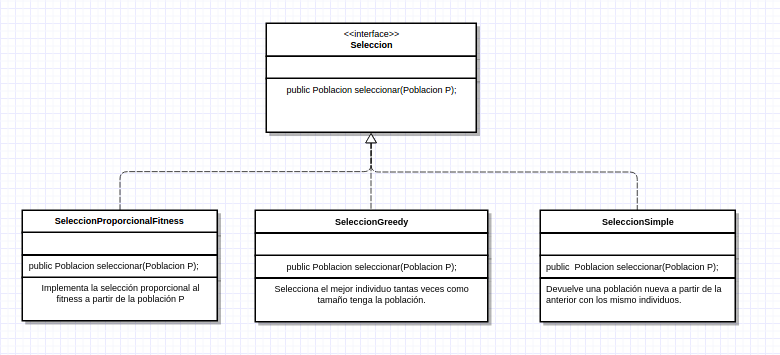
\includegraphics[scale=0.5]{img/SeleccionUML.png}
\end{center}

Hemos implementado 3 formas de selección. Cada clase simplemente implementa el método seleccionar de una manera distinta. A continuación, describimos los métodos implementados en cada clase.

\begin{itemize}
 	\item \textit{SelccionSimple.java}: Implementada primera para la fase de pruebas. Es tan simple como devolver una población igual que la recibida.
 	\item \textit{SeleccionProporcionalFitness.java}: el método sugerido por el enunciado visto en clase de teoría.
 	\item \textit{SeleccionGreedy.java} Una selección avariciosa que crea una nueva población con todos sus individuos iguales al mejor de la recibida como argumento.
 \end{itemize}  


 El análisis sobre los resultados obtenidos con un método de selección u otro se encuentra en la sección de resultados (\ref{sec:Resultados}) 


\subsection{Reemplazo}
A continuación, incluimos el diagrama de clases que hemos utilizado.


\begin{center}
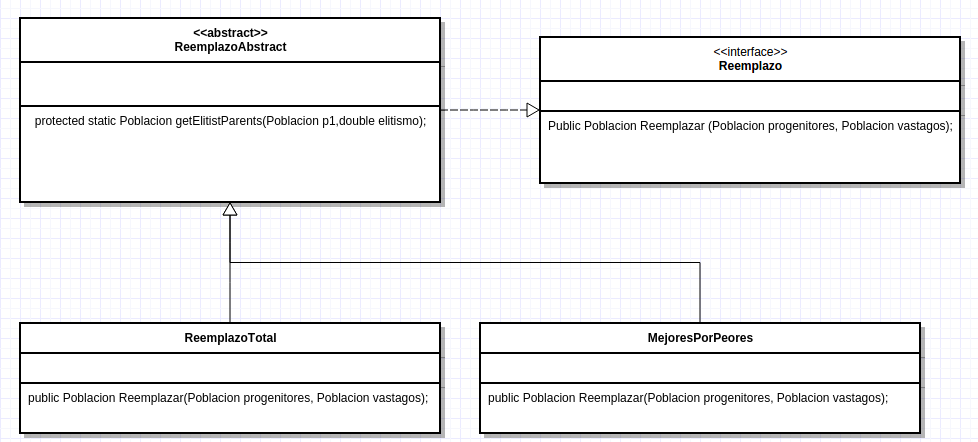
\includegraphics[scale=0.4]{img/ReemplazoUML.png}
\end{center}

La necesidad de la clase abstracta intermedia es que en la versión de Java utilizada (1.7) no es posible incluir implementaciones de métodos en una interfaz\footnote{En la siguiente versión de Java (1.8) sí es posible, pero hemos preferido utilizar la versión 1.7, creando esta clase abstracta intermedia para evitar problemas de compatibilidad}. Es por ello que incluimos la clase abstracta intermedia \texit{ReemplazoAbstract.java} con un método para seleccionar un porcentaje de la población (pensando para la selección de la élite de la población).

De esta manera, todas las maneras de reemplazar implementan de la misma manera el elitismo.

Como se aprecia en el diagrama, hemos implementado 2 clases, cada una con un método de reemplazo distinto.

\begin{itemize}
	\item \textit{ReemplazoTotal.java} implementa el reemplazo natural. Los hijos sustituyen a los padres. En caso de utilizar elitismo (sea $p$ el porcentaje de elitismo), la población resultante del reemplazo tendrá $p\%$ de padres y $(100-p)\%$ de hijos.
	\item \textit{MejoresPorPeores.java} implementa el reemplazo que pensamos que debería ser óptimo. Se juntan las 2 poblaciones (padres e hijos) y se seleccionan los $n$ mejores individuos (donde $n$ es el tamaño de la población). 
	\subitem En caso de implementar elitismo (sea $p$ el porcentaje de elitismo), la población resultante incluirá $p\%$ de padres (independientemente de que estos sean mejores que los hijos).
\end{itemize}

El análisis sobre los resultados obtenidos con un método de selección u otro se encuentra en la sección de resultados (\ref{sec:Resultados}) 


\chapter{Resultados}
\section{Tabla de resultados}

A continuación incluimos la tabla con todos los resultados obtenidos (para individuos de 11 reglas).

\begin{center}
\begin{tabular}{cccc|c}
Reemplazo & Seleccion & Poblacion & Generaciones & Error\\\hline
ReemplazoTotal & SeleccionProporcionalAlFitness & 10 & 100 & \textcolor{red}{34.769\%} \\
ReemplazoTotal & SeleccionProporcionalAlFitness & 10 & 350 & 26.769\% \\
ReemplazoTotal & SeleccionProporcionalAlFitness & 100 & 100 & 31.077\% \\
ReemplazoTotal & SeleccionProporcionalAlFitness & 100 & 350 & 26.154\% \\
ReemplazoTotal & SeleccionProporcionalAlFitness & 500 & 100 & 24.615\% \\
ReemplazoTotal & SeleccionProporcionalAlFitness & 500 & 350 & \textcolor{green}{23.692\%} \\
\end{tabular}
\end{center}

\begin{center}
\begin{tabular}{cccc|c}
Reemplazo & Seleccion & Poblacion & Generaciones & Error\\\hline
ReemplazoTotal & SeleccionProporcionalAlFitness & 73 & 73 & 26.769\% \\
ReemplazoTotal & SeleccionAvariciosa & 73 & 73 & 29.846\% \\
ReemplazoTotal & SeleccionSimple & 73 & 73 & 31.692\% \\
MejoresPorPeores & SeleccionProporcionalAlFitness & 73 & 73 & 31.385\% \\
MejoresPorPeores & SeleccionAvariciosa & 73 & 73 & 31.077\% \\
MejoresPorPeores & SeleccionSimple & 73 & 73 & 26.154\% \\
\end{tabular}
\end{center}




\section{Análisis de resultados}
\label{sec:Resultados}

\subsection{Importancia del número de Reglas}
\label{subsec:numReglas}

El número de reglas es un factor muy importante. Si tenemos una única regla, será muy poco probable que los datos a clasificar la cumplan y por lo tanto asignaremos la clase por defecto a prácticamente todos los datos, provocando una clasificación muy sesgada. En caso de tener demasiadas reglas a las que asignamos una clase, es fácil que los datos a clasificar cumplan alguna de esas reglas (por las disyuntivas de las reglas). Por otro lado, al tener muchas reglas, hay más posibilidades de que se generen a partir de mutaciones y cruces las reglas óptimas.

Por ello, hemos tomado 2 decisiones. La primera es el estudio de la importancia del número de regla, utilizando un número fijo de reglas para todos los individuos. Además, el número de reglas utilizado en el análisis de los resultados ha sido variable,  dando lugar a una mejor algoritmo de esta manera.

A continuación, la tabla de los resultados del estudio de la importancia del número de reglas.

\begin{center}
\begin{tabular}{cc}
Reglas&Error\\\hline
5 & 29.846\%\\
11 & 22.462\%\\
16 & 31.077\%\\
25 & 27.692\%\\
50 & 68.923\%\\
150 & 64.615\%\\
\end{tabular}
\end{center}
Los par\'amemtros utilizados han sido:\begin{itemize}
\item \#Individuos: 75 \item Generaciones: 75 \item Elitismo: 5.00\%\item PCruce: 60.00\%\item PMut: 1.00\%\item Reemplazo: SeleccionProporcionalAl\item Selecci\'on: MejoresPorPeores
\end{itemize}


Vemos que es un factor influyente. Por estos resultados es por los que hemos elegido un número inicial de reglas = 11 (aunque lo que sugería el enunciado era cercano a 25).

Aun así, hemos preferido un número variable de reglas. 

\section{Evolución del fitness}



\end{document}
